\section{Decoupling of Flow and Congestion Control}
As mentioned earlier, Viscous decouples congestion and flow control, where congestion control is associated with the channel layer, and flow control is associated with the flow layer. The flow control algorithm uses the receiver advertised window size ($rwnd$) to control the rate of traffic flows from the application, so that the traffic generation rate from the source application does not overshoot the traffic reception rate at the target application. The interesting design choice for Viscous is that if there is congestion in one of the paths among all the available ones, the traffic generation rate from the application may not need to be dropped down when other paths (or channels) have sufficient bandwidth. However, when congestion is severe (there is congestion in more than one paths), that feedback needs to be passed to the flow control module so that the application traffic generation rate can be shaped accordingly to avoid data overflow from the Viscous packet buffer. Therefore, we design the following approach for decoupled flow and congestion controls in Viscous. 
%Here we will try to find the relation between flow-control and congestion-control.

\subsection{Mesuring mean throughput achieved by a channel}
At first we try to model expected congestion window size ($cwnd$) in steady state condition for a single channel. We  follow the modeling provided in \cite{Padhye2000}. Here we assumes that in steady state, available bandwidth is almost constant. RTT varies only because of the queuing delay. Also, links are lossless and packets get dropped due to buffer overflow at the different queues i.e. packet loss are the signal for congestion in the path.

As mentioned in the earlier section, the congestion control algorithm has five states which are {\it Slow Start}, {\it Congestion Avoidance}, {\it Fast Retransmit}, {\it Fast Recovery}, {\it Multi Recovery} and {\it Timeout}. Among them {\it Fast Retransmit} and {\it Timeout} are very brief to affect anything to have any effect on the mean $cwnd$ however require to transmit the lost packets immediately.

\begin{figure}[!h]
	\centering
	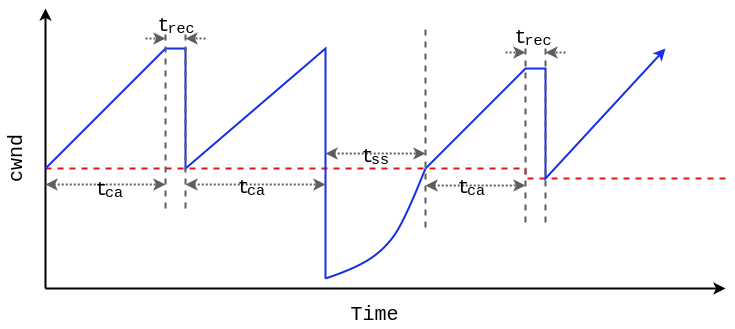
\includegraphics[width=\linewidth]{img/model/window_evolution}
	\caption{Theoretical steady state window evolution by the proposed congestion control algorithm.}
	\label{fig:cwnd-evo}
\end{figure}

In Fig.~\ref{fig:cwnd-evo}, we have shown $cwnd$ evolution in steady-state for a Viscous channel. Here, $cwnd$ starts from $ssthresh$ and the Viscous channel is in {\it Congestion Avoidance} state. $cwnd$ grows upto $cwnd_{max}$ for $t_{ca}$ duration till sender receives a three duplicate ACKs (DUP). Then it spends in {\it Fast Retransmission} state for a very brief time and moves to {\it Fast Recovery} state. It may happen that the Viscous channel moves to {\it Multi Recovery} state. However, there are no change in congestion window $cwnd$ until it get out of the recovery state. Total duration it have to spent in the recovery state for $t_{rec}$ time.

In steady-state, timeout may occur for some packets. In that case, the Viscous channel moves to {\it Slow Start} state and spends $t_{ss}$ duration before it moves to the {\it Congestion Avoidance} state. Now, let the probability of spending time at {\it Congestion Avoidance} state be $p_{ca}$ and probability of spending time at {\it SlowStart} state be $p_{ss}$.

\begin{equation} \label{eqn:cwnd_update}
cwnd_{i+1} = 	
\begin{cases}
 2 \times cwnd_{i} & \text{\it SlowStart} \\
 cwnd_{i} + 2 & \text{\it Congestion Avoidance} \\
 cwnd_{i} / 2 & \text{On three DUP ACK} \\
 1 & \text{On timeout event} 
\end{cases}
\end{equation}

Now, there are several way congestion window ($cwnd$) updates as per the Eqn.~\ref{eqn:cwnd_update}, i.e. it doubles the $cwnd$ per RTT during the {\it Slow Start} state and increases by 1 packet per RTT in the {\it Congestion Avoidance} state. Upon receipt of three duplicate ACKs, $cwnd$ set to half and after a timeout, it set $cwnd$ to 1.
Upon receipt of three duplicate ACKs, a Viscous channel spent some time in recovery state ({\it Fast Recovery} and {\it Multi Recovery}). During this period, effective $cwnd$ does not change. The Viscous channel stays in {\it Congestion Avoidance} state for $t_{ca}$ time, $t{rec}$ time in recovery state and $t_{ss}$ time in {\it Slow Start} state.


Now, the average congestion window ($cwnd$) during {\it Slow Start}($cwnd_{avg_{ss}}$), {\it Congestion Avoidance} ($cwnd_{avg_{ca}}$), and Recovery ($cwnd_{avg_{rec}}$) states are

\begin{equation}
\begin{split}
cwnd_{avg_{ss}} &= \frac{\int\limits_{0}^{t_{ss}} 2^x dx}{t_{ss}} \\
&= \frac{2^{t_{ss}}-1}{t_{ss} \times \ln{2}}
\end{split}
\end{equation}

\begin{equation}
\begin{split}
cwnd_{avg_{ca}} = ssthresh + \frac{1}{2}t_{ca}
\end{split}
\end{equation}

\begin{equation}
\begin{split}
	cwnd_{avg_{rec}} = t_{ca}+ssthresh
\end{split}
\end{equation}

Recovery state happens only after three duplicate ACKs, but not after a timeout. So, in the steady states, it is recovery state or {\it Slow Start} state after a {\it Congestion Avoidance} state. So, we need to find out the mean $cwnd$ for (a) {\it Congestion Avoidance} state followed by a recovery state (i.e. $cwnd_{avg_{ca+rec}}$) and for (b) {\it Congestion Avoidance} state followed by a {\it SlowStart} (i.e. $cwnd_{avg_{ca+ss}}$) (Fig.~\ref{img:cong-state-tran}).

\begin{equation}
\begin{split}
&cwnd_{avg_{ca+rec}} \\
&= \frac{cwnd_{avg_{ca}} \cdot t_{ca} + cwnd_{avg_{rec}} \cdot t_{rec}} {t_{ca} + t_{rec}} \\
&= \frac{\frac{1}{2} t_{ca}^2+ssthresh \cdot t_{ca} + (t_{ca}+ssthresh) \cdot t_{rec}}{t_{ca} + t_{rec}} \\
&= \frac{1}{2} \cdot \frac{t_{ca}^2}{t_{ca} + t_{rec}} + \frac{t_{ca} \cdot t_{rec}}{t_{ca} + t_{rec}} + \frac{2 \cdot ssthresh}{t_{ca} + t_{rec}}
\end{split}
\end{equation}

\begin{equation}
\begin{split}
cwnd_{avg_{ca+ss}} &= \frac{cwnd_{avg_{ca}} \cdot t_{ca} + cwnd_{avg_{ss}} \cdot t_{ss}} {t_{ca} + t_{ss}} \\
&= \frac{\frac{1}{2} t_{ca}^2+ssthresh \cdot t_{ca} + \frac{2^{t_{ss}}-1}{\ln{2} \cdot t_{ss}} \cdot t_{ss}}{t_{ca} + t_{ss}} \\
\end{split}
\end{equation}


We assume that the probability of occurrence of timeout is $p$ and probability of triple DUP is ($1-p$). So, the average congestion window $cwnd_{avg}$ for a single Viscous channel.
\begin{equation}
\begin{split}
cwnd_{avg} = p \cdot cwnd_{avg_{ca+ss}} + (1-p) \cdot cwnd_{avg_{ca+rec}}
\end{split}
\end{equation}

This is same for all the channel available in a Viscous connection. So, we can write that average congestion window size in steady state for $i^{th}$ channel is $cwnd_{avg_i}$.

Till now, we measured the time with respect to a RTT. Let us assume that the mean RTT of the channel $i$ is $rtt_{m_i}$. Then throughput $B_i$ of the channel is, 
\begin{equation}
B_i = \frac{cwnd_{avg_i}}{rtt_{m_i}}
\end{equation}


So, the overall throughput $\mathcal{B}$ of a Viscous connection is:
$$ \mathcal{B} = \sum_{i}^{} B_i = \sum_{i}^{} \frac{cwnd_{avg_i}}{rtt_{m_i}} $$


However, it is the maximum throughput we can get from the channel layer where there is no flow control applied. Now, if we consider Flow layer, our system looks like Fig.~\ref{fig:sys_que}. Here we have $n$ flows in flow layer. Scheduler collect data from flow as scheduling policy and bandwidth available at channel layer. There can be multiple channel in the system, each channel can transmit data reliably to a remote host.

\begin{figure}[!h]
	\centering
	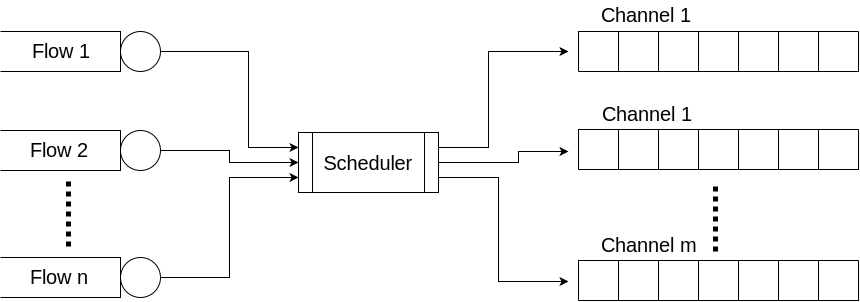
\includegraphics[width=\linewidth]{img/model/system_queue}
	\caption{Queuing diagram.}
	\label{fig:sys_que}
\end{figure}

\begin{algorithm*}[!ht]
	\SetKwFunction{findAllocation}{findAllocations}
	\nonl\findAllocation{$\mathcal{B}, \mathcal{X}, \mathcal{W}$}\\
	\KwData{$\mathcal{B} \gets \text{ available bandwidth}$ \\
				$\mathcal{X} \gets \{\mathcal{X}_1, \mathcal{X}_2 ... \mathcal{X}_n \}$ \\
				$\mathcal{W} \gets \{w_1, w_2 ... w_n\} $
				}
	\KwResult{$\mu \gets \{\mu_1, \mu_2 ... \mu_n\}$}
	\Indp
	\If{$|X| == 0$}{\Return{\{\}}}
	$\mu^s \gets \{\}$ //sets where $\mathcal{X}_i < \frac{w_i}{\sum_{\forall j}w_j} \mathcal{B}$\\
	$\mu^h \gets \{\}$ //sets where $\mathcal{X}_i \ge \frac{w_i}{\sum_{\forall j}w_j} \mathcal{B}$ \\
	\ForAll{$\mathcal{X}_i \in \mathcal{X}$}{
		$\mu_i \gets \frac{w_i}{\sum_{\forall j}w_j} \mathcal{B}$ \\
		\If{$\mu_i > \mathcal{X}_i$}{
			$\mu^s \gets \mu^s \cup \{\mathcal{X}_i\}$ \\
		}
		\Else{$\mu^h \gets \mu^h \cup \{\mu_i\}$}
	}
	\If{$|\mu^h| = |\mathcal{X}|$}{
		$\mu \gets \mu^h$ \\
		\Return $\mu$
	}
	\If{$|\mu^s| = |\mathcal{X}|$}{
		$\mu \gets \mu^s$ \\
		\Return $\mu$
	}
	
	$\mu \gets \mu^s$
	
	$\mathcal{B}' \gets \mathcal{B} - \sum_{ \mu_i \in \mu} \mu_i$ \\
	$\mathcal{X}' \gets \mathcal{X} \setminus \{\mathcal{X}_i | \forall_i \mu_i \notin \mu\}$ \\
	$\mathcal{W}' \gets \mathcal{W} \setminus \{w_i | \forall_i \mu_i \notin \mu\}$ \\

	$\mu \gets \mu\ \cup$ \findAllocation{$\mathcal{B}', \mathcal{X}', \mathcal{W}'$}\\
	\Return{$\mu$}
\caption{\label{algo:findTheBandwidth} Finding best bandwidth allocation based on the weights}
\end{algorithm*}


%\subsection{Scheduling}
Flow layer sends packets to the scheduler, and the scheduler schedules packets to the channels. The maximum arrival rate at the scheduler from the all flows can be $\mathcal{B}$ i.e. cumulative bandwidth of the channels. The scheduler schedules packets from $i^{th}$ flow with weight $w_i$. $w_i$ is an integer with minimum value 1. For rest of the part, we accumulated meaning of different symbols in Table~\ref{table:proofsymbols}.

\begin{table}
	\centering
	\begin{tabular}{|rl|}
		\hline
		$\mathcal{B} =$& Cumulative mean bandwidth available in all channels. \\
		$f_i =$& $i^{th}$ flow. \\
		$\mathcal{F} =$& Set of available flows in the viscous connection. \\
		$w_i =$& Weight of the flow $f_i$. It is integer with minimum value 1. \\
		$\mathcal{W} =$& Set of $w_i$ for all flows.\\
%		$\mathcal{P}_i=$& $\frac{w_i}{\sum_{i} w_i}$ \\
		$\lambda_i =$& Data generation rate at application for the flow $f_i$. \\
		$r_i =$& Maximum flow rate controlled receiver's window.\\
		$\mathcal{X}_i =$& $\min(r_i, \lambda_i)$\\
		$\mathcal{X} =$& Set of $\mathcal{X}_i$ for all flows.\\
		$\mu_i =$& Allocated bandwidth to flow $f_i$.\\
		$\mathcal{\mu} =$& Set of allocated bandwidth.\\
		\hline
	\end{tabular}
	\caption{\label{table:proofsymbols}List of symbols}
\end{table}

Each flow has two independent parameters, (a) data generation rate ($\lambda_i$) from the application and (b) flow rate ($r_i$) controlled by the receiver's window. So, a flow can send data at most $\mathcal{X}_i = \min(\lambda_i, r_i)$. The scheduler needs to allocate bandwidth $\mu_i$ from the available bandwidth $\mathcal{B}$ as per their weight $w_i$ i.e $\mu_i = w_i \cdot \mathcal{B}/\sum_{w_j}w_j$. The scheduler also do not want to keep channels under-utilized. In case, for some flow $f_i$, $\mathcal{X}_i < w_i \cdot \mathcal{B}/\sum_{w_j}w_j$, scheduler allocates $\mu_i = \mathcal{X}_i$ only and distributes surplus to other flow as per their weights. The bandwidth problem boils down to Proportional Fairness problem described by Kelly {\it et. al.} in \cite{Kelly1998}. Here we can describe our problem as the following optimization problem:

{\bf Objective:} $$\max \sum_{\forall i \in F} w_i \log \mu_i$$

{\bf Subjected to } $$\sum_{\forall_i \in F}\mu_i \le \mathcal{B}$$
{and} $$\mu_i \le \mathcal{X}_i \ \ \ \ \ \ \ \forall_i \in F$$

\subsection{Calculating a Feasible Allocation Vector}
Solution to this problem is as follows: $$\mu = F(\mathcal{B}, \mathcal{W}, \mathcal{X})$$

\begin{equation}
\label{eqn:formula}
F(\mathcal{B}, \mathcal{W}, \mathcal{X}) = 
\begin{cases}
\Phi & \text{if } |\mathcal{X}| == 0 \\ 

\{\mu_i = \frac{w_i}{\sum_{\forall j}w_j} \mathcal{B} | \forall_i\} 
& \text{if } \forall_i \mathcal{X}_i \ge \frac{w_i}{\sum_{\forall j}w_j} \mathcal{B} \\

\{\mu_i = \mathcal{X}_i\ | \forall_i \mathcal{X}_i \le \frac{w_i}{\sum_{\forall j}w_j} \mathcal{B} \} \cup F(\mathcal{B}', \mathcal{W}', \mathcal{X}') 
	& \text{Otherwise}
%	\ \ \hfill \text{if } \exists_i \mathcal{X}_i \le \frac{w_i}{\sum_{\forall j}w_j} \mathcal{B} \text{ and } \exists_i \mathcal{X}_i > \frac{w_i}{\sum_{\forall j}w_j} \mathcal{B}
\end{cases} \\
\end{equation}
While 
$$\mathcal{B}' = \mathcal{B} - \sum_{\forall_i \mathcal{X}_i \le \frac{w_i}{\sum_{\forall j}w_j} \mathcal{B}} \mathcal{X}_i$$
$$\mathcal{W}' = \mathcal{W} \setminus \{w_i | \forall_i \mathcal{X}_i \le \frac{w_i}{\sum_{\forall j}w_j} \mathcal{B} \}$$
$$\mathcal{X}' = \mathcal{X} \setminus \{\mathcal{X}_i | \forall_i \mathcal{X}_i \le \frac{w_i}{\sum_{\forall j}w_j} \mathcal{B}\})$$

%The Algorithm~\ref{algo:findTheBandwidth} provides a solution to the given recurrence in Eqn.~\ref{eqn:formula}.

\begin{theorem}
	The Algorithm~\ref{algo:findTheBandwidth} that solves eqn.~(\ref{eqn:formula}) gives the optimal solution for the optimization problem.
\end{theorem}

The allocation vector $\mu$ provided by the Algorithm~\ref{algo:findTheBandwidth}. As described in \cite{Kelly1998} by Kelly {\it et. al.}, $\mu$ is optimal iff for any feasible $\mu^*$, eqn~(\ref{eqn:proofeqn}) satisfy.

\begin{equation}
\label{eqn:proofeqn}
\sum_{\forall i} w_i \frac{\mu_i^* - \mu_i}{\mu_i} \le 0
\end{equation}

{\bf Proof}: The Algorithm~\ref{algo:findTheBandwidth} and Eqn.~(\ref{eqn:formula}) returns allocation $\mu$. It allocates available bandwidth among flows according to their weight and minimizes the bandwidth wastage. We can see that the algorithm allocates $\mathcal{X}_i$ to $i^{th}$ flow if possible and passes the surpass to next iteration to allocate accordingly based on the weights for rest of the flows. So, among $n$ flows, the algorithm allots $k$ flows to $\mathcal{X}_i$ and rest of the flows according to weight with remaining bandwidth. So, $$\mu = \{\mathcal{X}_1, \mathcal{X}_2, ... \mathcal{X}_k, \mu_{k+1}, ..., \mu_{n}\}$$ where $$\mu_i = \frac{w_{i}}{\sum_{j=k+1}^{n}w_j}(\mathcal{B} - \sum_{j=1}^{k}\mathcal{X}_i) \ \ \ \ for\ i=k+1,k+2,...,n$$

%Now, we want to proof $\mu$ is optimal using proof by contradiction. For the shake of contradiction, lets assume there exists some $\mu^* = \{\mu_i+\epsilon_i | \forall_i\}$ for which $$\sum_i w_i \frac{\mu_i^* - \mu_i}{\mu_i} > 0$$

To prove that our algorithm provides optimal solution, we have to prove three different cases depending on the value of $k$. These cases are ii) $k = 0$, ii) $0 < k < n$ and iii)$k = n$. These three cover all possible combination as it covers the range of $k$ ({\it i.e.} $0 \le k \le n$).

{\bf Case i:} When $k=0$, $\mu_i = \frac{w_i}{\sum_{j}w_j}\mathcal{B}$

Here, it is observed that $\sum_i \mu_i = \mathcal{B}$ and for any other feasible solution $\mu^* = \{\mu_i^* = \mu_i+\epsilon_i | \forall_i\}$, as per the constraints $\sum_i \mu_i^* \le \mathcal{B}$.

%\begin{equation}
%\begin{split}
%\sum_i \mu_i^* - \sum_i \mu_i \le& \ \mathcal{B} - \mathcal{B}\\
%\sum_i (\mu_i^* - \mu_i) \le& \ 0\\
%\sum_i \epsilon_i \le& \ 0
%\end{split}
%\end{equation}

%Now, 

\begin{equation}
\begin{split}
&\sum_i w_i \frac{\mu_i^* - \mu_i}{\mu_i} \\
&= \sum_i w_i \frac{\mu_i^* - \mu_i}{\frac{w_i}{\sum_{j}w_j} \mathcal{B}} \\
&= \sum_i  \frac{\sum_{j}w_j \cdot (\mu_i^* - \mu_i)}{\mathcal{B}} \\
&= \frac{\sum_{j}w_j}{\mathcal{B}} \sum_i (\mu_i^* - \mu_i)\\
&= \frac{\sum_{j}w_j}{\mathcal{B}} \left( \sum_i \mu_i^* - \sum_i \mu_i \right) \\
&\le 0 \\
& \omit \hfill \text{$\sum_i \mu_i^* \le \mathcal{B}$} \\
\end{split}
\end{equation}
$\mu$ is optimal for this case also.

{\bf Case ii:} When $0<k<n$
Here
\begin{equation}
\label{eqn:case3-1}
\begin{split}
\mu_i =& \mathcal{X}_i \\ & \omit\hfill \text{} i=1,2,...,k \\
\mu_i =& \frac{w_i}{\sum_{j=k+1}^{n} w_j} \left(\mathcal{B}-\sum_{j=1}^{k}\mathcal{X}_j\right) \\ & \omit\hfill \text{} i=k+1,k+2,...,n\\
\end{split}
\end{equation}

Our algorithm returns allocation $\mu$ where allocation for few flows are saturated (i.e. $\mu_i = \mathcal{X}_i$) and it is unsaturated for other flows. In every iteration, algorithm first try to distribute available bandwidth to every unsaturated flows. In this process, if any flows get saturated and have some surpass, algorithm go for next iteration and distribute the surpass among the unsaturated flow according to their weight. If surpass bandwidth in a iteration $x$ is $\mathcal{B}_{r_x}$ and the sum of weight of unsaturated flows in the same iteration $x$ is $\mathcal{W}_{s_x}$ then bandwidth allocation for $i^{th}$ flow which is unsaturated, in iteration $x$, will be $\mu_i = \min\left( \mu_i + w_i\frac{\mathcal{B}_{r_x}}{\mathcal{W}_{s_x}}, \mathcal{X}_i \right)$. So we can write that for a saturated flow $i$ 
\begin{equation}
\label{eqn:case3-2}
\begin{split}
\mu_i \le& w_i \left( \frac{\mathcal{B}}{w_{s_0}} + \frac{\mathcal{B}_{r_1}}{w_{s_1}} + \frac{\mathcal{B}_{r_2}}{w_{s_2}} + ... + \frac{\mathcal{B}_{r_m}}{w_{s_m}} \right) \\ 
& \omit\hfill \text{} i=1,2,...,k \\
\end{split}
\end{equation}

For a unsaturated flow $i$
\begin{equation}
\label{eqn:case3-3}
\begin{split}
\mu_i =& w_i \left( \frac{\mathcal{B}}{w_{s_0}} + \frac{\mathcal{B}_{r_1}}{w_{s_1}} + \frac{\mathcal{B}_{r_2}}{w_{s_2}} + ... + \frac{\mathcal{B}_{r_m}}{w_{s_m}} \right) 
\\ & \omit\hfill \text{} i=k+1,k+2,...,n\\
\end{split}
\end{equation}


We already know that $\sum_{i=1}^{n} \mu_i = \mathcal{B}$. We can also say that for any feasible allocation  $\sum_{i=1}^{n} \mu_i^* \le \mathcal{B}$. Now, $\mu$ has allocated bandwidth for $k$ flows to $\mathcal{X}_i$ which saturate there allocation. So, for any other feasible allocation, these $k$ flow can not be allocated more that. But, for rest of the flows, which have unsaturated allocation, can be allocated more. So, we can write that $\mu^* = \{\mu_i^* = \mu_i - \epsilon_i | i=1,2,...,k\}\cup\{\mu_i^* = \mu_i - \epsilon_i | i=k+1,k+2,...,n\}$

\begin{equation}
\label{eqn:case3-4}
\begin{split}
&\sum_{i=1}^{n} \mu_i^* - \sum_{i=1}^{n} \mu_i \le 0 \\
\implies & \sum_{i=1}^{k} \mu_i^* + \sum_{i=k+1}^{n} \mu_i^* - \left( \sum_{i=1}^{k} \mu_i + \sum_{i=k+1}^{n} \mu_i \right) \le 0 \\
\implies & \sum_{i=1}^{k} (\mu_i^* - \mu_i) + \sum_{i=k+1}^{n} (\mu_i^* - \mu_i) \le 0 \\
\implies & \sum_{i=1}^{k} -\epsilon_i + \sum_{i=k+1}^{n} \epsilon_i \le 0 \\
\end{split}
\end{equation}



Now, we can expand the Equation~(\ref{eqn:proofeqn}) as follows:

\begin{equation}
	\begin{split}
	& \sum_{i=1}^{n} w_i \frac{\mu_i^* - \mu_i}{\mu_i} \\
	=& \sum_{i=1}^{k} w_i \frac{\mu_i^* - \mu_i}{\mu_i} + \sum_{i=k+1}^{n} w_i \frac{\mu_i^* - \mu_i}{\mu_i} \\
	=& \sum_{i=1}^{k} w_i \frac{-\epsilon_i}{\mu_i} + \sum_{i=k+1}^{n} w_i \frac{\epsilon_i}{\mu_i}\\
	=& \sum_{i=1}^{k} w_i \frac{\epsilon_i}{-\mu_i} + \sum_{i=k+1}^{n} w_i \frac{\epsilon_i}{\mu_i}\\
	\le & \sum_{i=1}^{k} w_i \frac{\epsilon_i}{- w_i \left( \frac{\mathcal{B}}{w_{s_0}} + \frac{\mathcal{B}_{r_1}}{w_{s_1}} + \frac{\mathcal{B}_{r_2}}{w_{s_2}} + ... + \frac{\mathcal{B}_{r_m}}{w_{s_m}} \right)} \\ 
%	& \omit\hfill \text{$\epsilon_i \le 0 $  for $i=1,2...k$}\\
	& + \sum_{i=k+1}^{n} w_i \frac{\epsilon_i}{w_i \left( \frac{\mathcal{B}}{w_{s_0}} + \frac{\mathcal{B}_{r_1}}{w_{s_1}} + \frac{\mathcal{B}_{r_2}}{w_{s_2}} + ... + \frac{\mathcal{B}_{r_m}}{w_{s_m}} \right)} \\
	& \omit\hfill \text{from Eqn.~(\ref{eqn:case3-2}) \& Eqn.~(\ref{eqn:case3-3})} \\
	&= \frac{1}{\left( \frac{\mathcal{B}}{w_{s_0}} + \frac{\mathcal{B}_{r_1}}{w_{s_1}} + \frac{\mathcal{B}_{r_2}}{w_{s_2}} + ... + \frac{\mathcal{B}_{r_m}}{w_{s_m}} \right)} \left( \sum_{i=1}^{k} -\epsilon_i + \sum_{i=k+1}^{n} \epsilon_i\right)  \\
	&\le 0\\
	& \omit\hfill \text{from Eqn.~(\ref{eqn:case3-4})}\\
	\end{split}
\end{equation}

We can say that for any feasible allocation $\mu^*$.
\begin{equation}
\begin{split}
\sum_{i=1}^{n} w_i \frac{\mu_i^* - \mu_i}{\mu_i} \le 0
\end{split}
\end{equation}


{\bf Case iii:} When $k=n$, $\mu = \{\mu_i = \mathcal{X}_i | \forall_i\}$.

As per the constraint of the optimization problem, the maximum value of any $\mu_i$ is $\mathcal{X}_i$, so, for any other feasible $\mu^*$, $\mu_i^* \le \mathcal{X}_i$. 
\begin{equation}
\begin{split}
&\sum_i \mu_i^* \le \sum_i \mu_i \\
%\implies &\sum_i \mu_i^* - \sum_i \mu_i \le 0 \\
%\implies &\sum_i \left( \mu_i^* - \mu_i \right) \le 0\\
\implies &\sum_i w_i \frac{ \mu_i^* - \mu_i }{\mu_i} \le 0 \\
\end{split}
\end{equation} 
$\mu$ is optimal for case 1.
\\



So, the solution given by our algorithm is optimal for every cases and it allows us to utilize maximum available bandwidth available for at the channel layer.
